In modern research in particles physics one approach of data acquisition is the collisions of acclerated particles, which interact during the collision via the known \gls{SM} interaction described in section \ref{sec:section_1_1} or possible unknown \gls{BSM} interactions. The products of interaction between can then be detected by analyzed by physicists. \\

In this thesis the data, which is analyzed for the search of \gls{LFV} in Z boson decays, is produced by proton-proton-collisions of the Large Hadron Collider (\gls{LHC}) \cite{LHC} and detected by the Compact Muon Solenoid (\gls{CMS}) \cite{CMS} in the year of 2016. Both apparatus are explained in the following sections, proton physics is explained in section \ref{sec:section_2_1_2}.


\section{Large Hadron Collider}
\label{sec:section_2_1}

The \gls{LHC} is a circular proton-proton-collider with a center of mass energy of $\sqrt{s} = 13$ tera electron volt (\gls{TeV}) \cite{LHC2}, which is located at the European Organization for Nuclear Research (\gls{CERN}) in Geneva. The accleration of the protons is done by a system and of pre-accelerators, which feeds the protons then in the \gls{LHC} to reach the designed center of mass energy, see figure \ref{fig:fig_2_1} for a schematic overview. \\

\begin{figure}[ht]
	\centering
	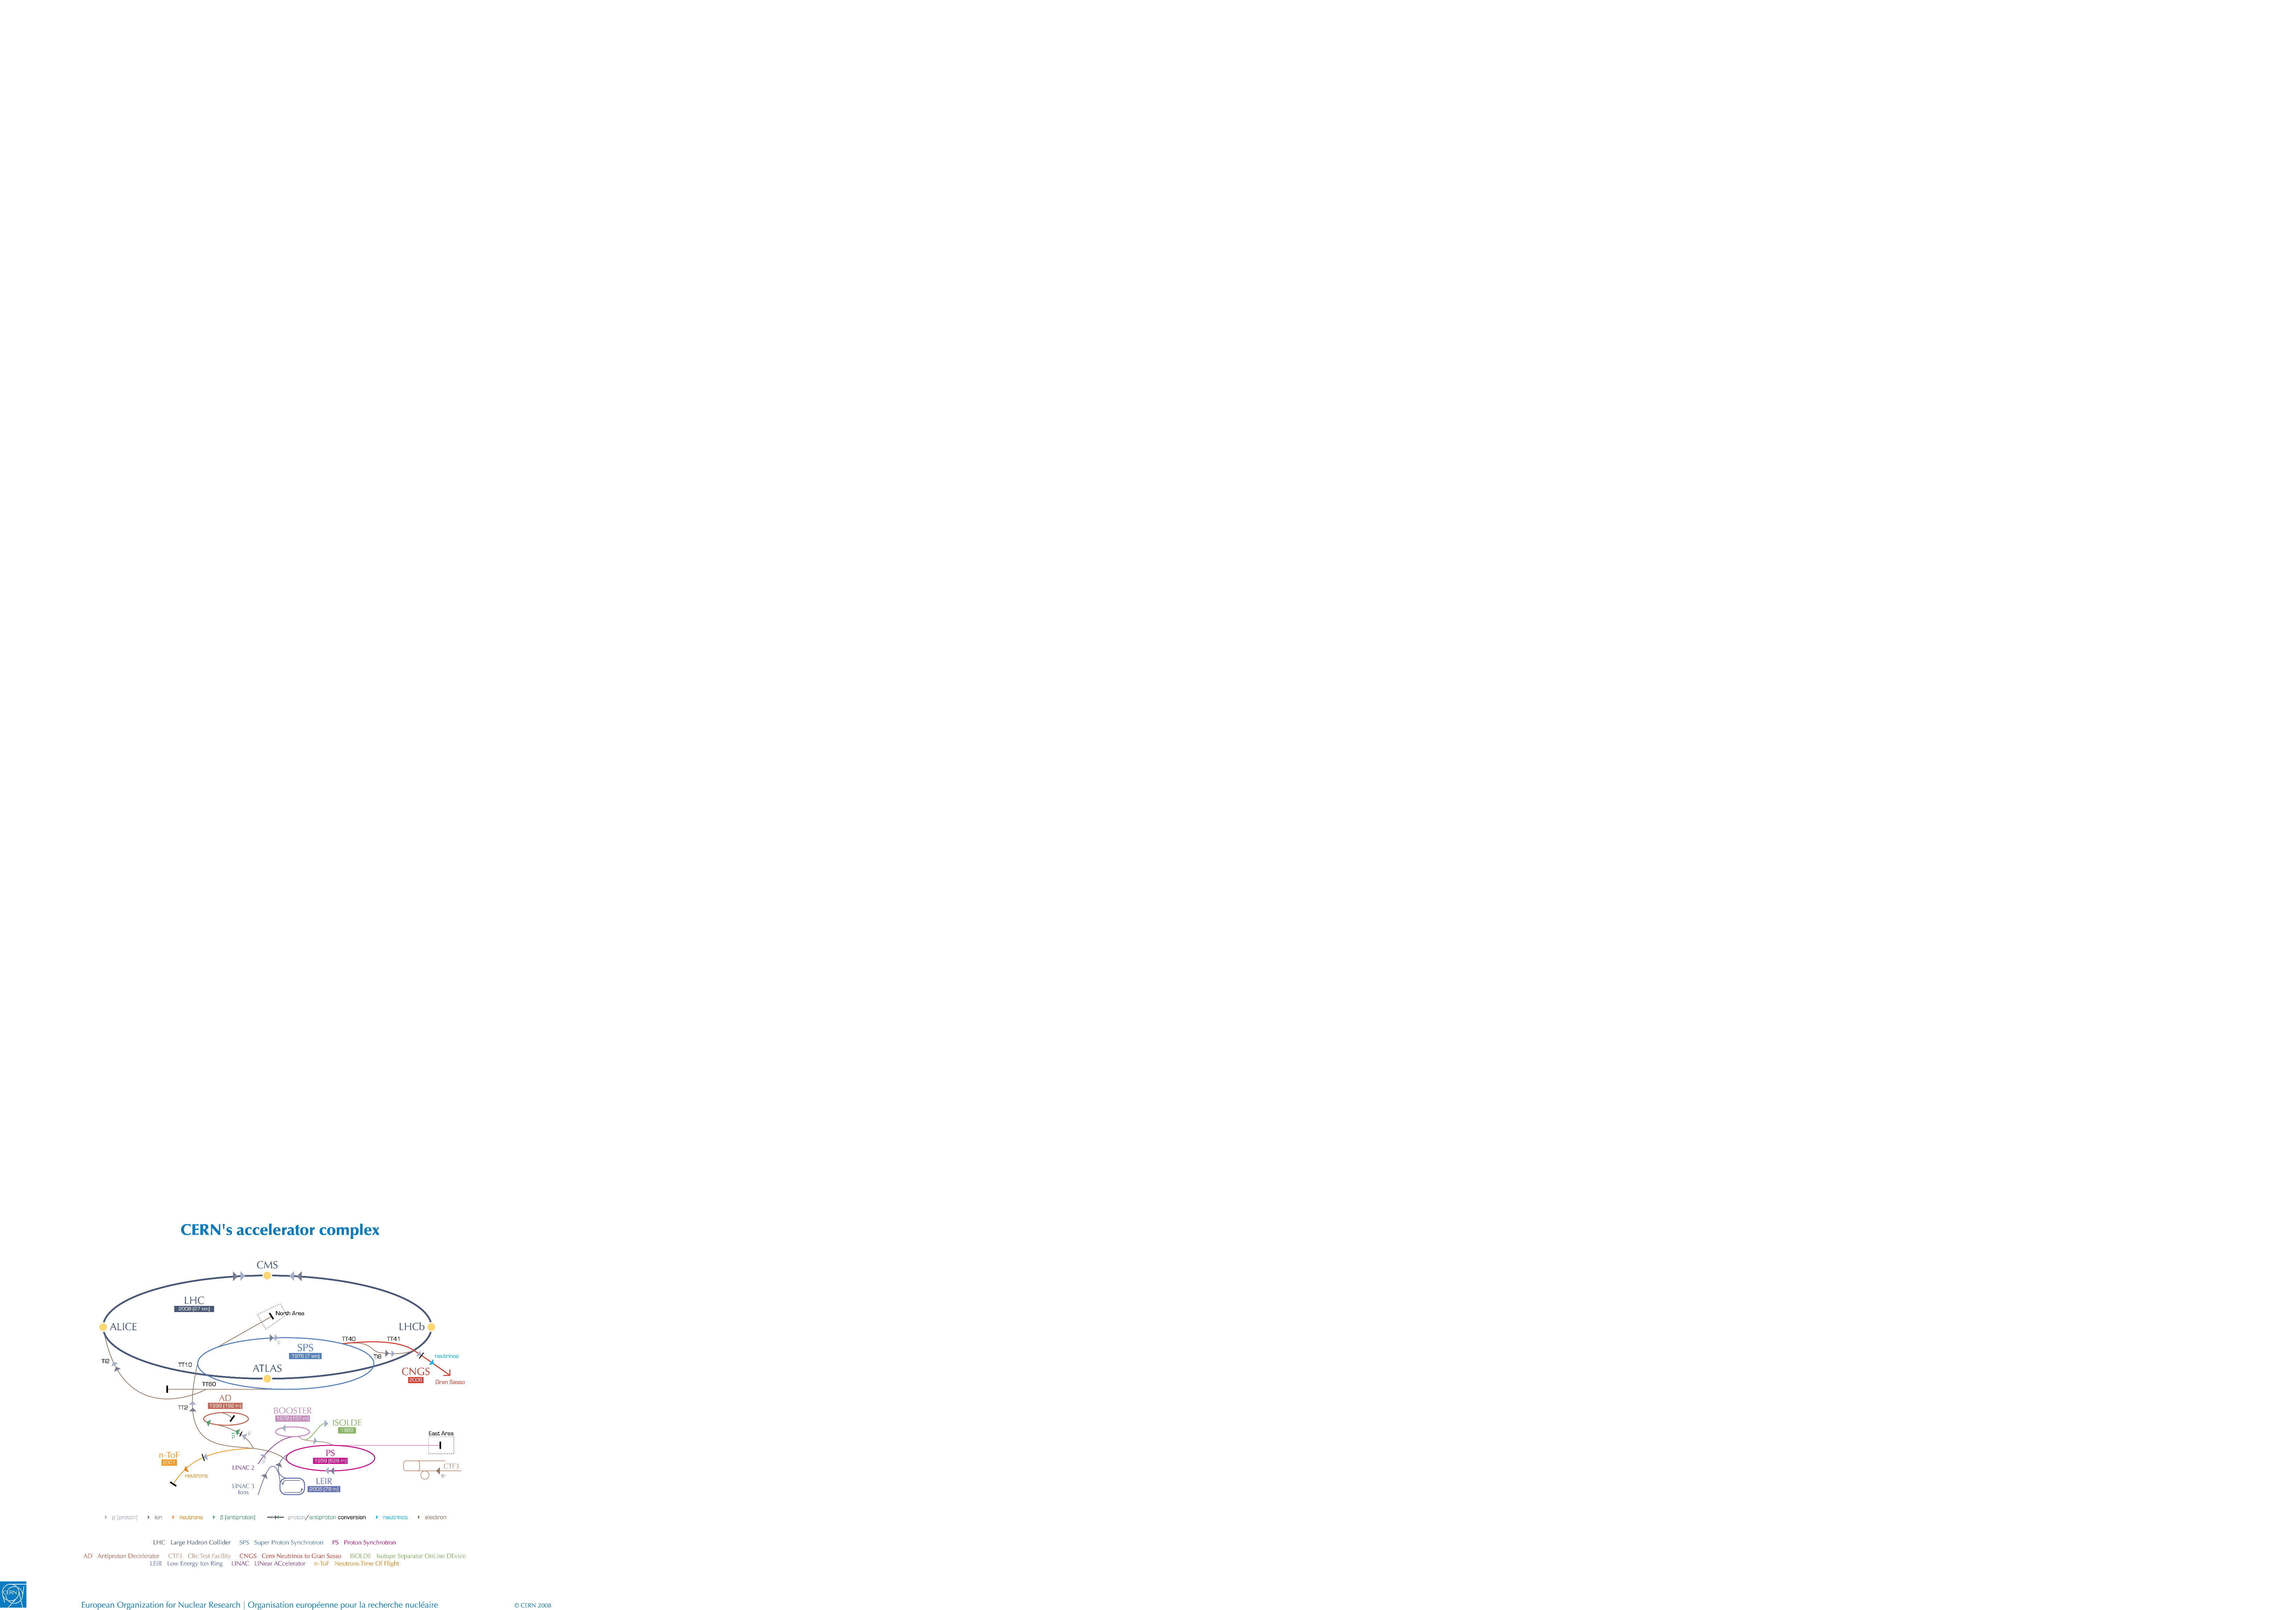
\includegraphics[width=1.0\textwidth]{pictures/LHC.pdf}

	\caption[Schematic overview of CERN accelerator complex]{Schematic overview of \gls{CERN} accelerator complex, including the \gls{LHC} and the previous pre-acclerators. The yellow points mark the position of the particles detectors at the collisions points. Taken from \cite{LHCACCL}}
	\label{fig:fig_2_1}
\end{figure}

At each collision point of the proton beams a sophisticated detector system is installed, indicated by the yellow dots in figure \ref{fig:fig_2_1}. Each of this detectors is designed for a special purpose of particle detection. The four big experiments are the \gls{CMS} and A Toroidal LHC Apparatus (\gls{ATLAS}) \cite{ATLAS}, which are designed to probe \gls{SM} and \gls{BSM} physics, the Large Hadron Collider beauty (\gls{LHCb}) \cite{LHCb}, which is designed for decays of hadrons, and the A Large Ion Collider Experiment (\gls{ALICE}) \cite{ALICE}, which is designed for heavy ion collisions.


\subsection{Properties of the proton beams}
\label{sec:section_2_1_1}

The protons in the \gls{LHC} are accelerated in so-called bunches, which contain around $10^{11}$ protons, and are seperated in space by a time interval of 25 ns \cite{LHCSTATS}. The size of the bunches is oscillating due to dynamics of the charged protons in the magnetic system of the \gls{LHC} \cite{LHC} and the beam size can be parametrized by the emittance $\epsilon$, which describe the cross section of the beam, and the $\beta$ function, which describes the oscillation amplitude \cite{BEAMPHY}. The properties of the beams has a high impact on the quality on the collider, which is parametrized by instantaneous luminosity $\mathcal{L}$ \cite{Luminosity}

\begin{equation}
	\label{eq:eq_2_1}
	\mathcal{L} = \frac{\gamma \cdot f \cdot k_{b} \cdot n_{1} \cdot n_{2}}{4 \cdot \pi \cdot \epsilon \cdot \beta}
\end{equation} 

with Lorentz gamma factor $\gamma$, the revolution frequency $f$ of the bunches, the number of colliding bunches $k_{b}$ and the number of protons $n_{i}$ in each bunch. There is a direct dependence of rate $\frac{dN}{dt}$ of collisions events to the luminosity, and the total number $N$ of collisions events to the integrated luminosity $\mathcal{L}_{int}$

\begin{equation}
	\label{eq:eq_2_2}
	\begin{split}
		\frac{dN}{dt} = \sigma \cdot \mathcal{L} \\
		N = \sigma \cdot \mathcal{L}_{int}
	\end{split}
\end{equation}	

with $\sigma$ as the cross section of proton-proton collisions. So the beam parameter have a direct influence on the total number of possible recorded events and the amount statistics which is provided for the analysis. Figure \ref{fig:fig_2_2} shows collected integrated luminosity of the data-taking run in 2016 in dependence of the day. 

\begin{figure}[ht]
	\centering
	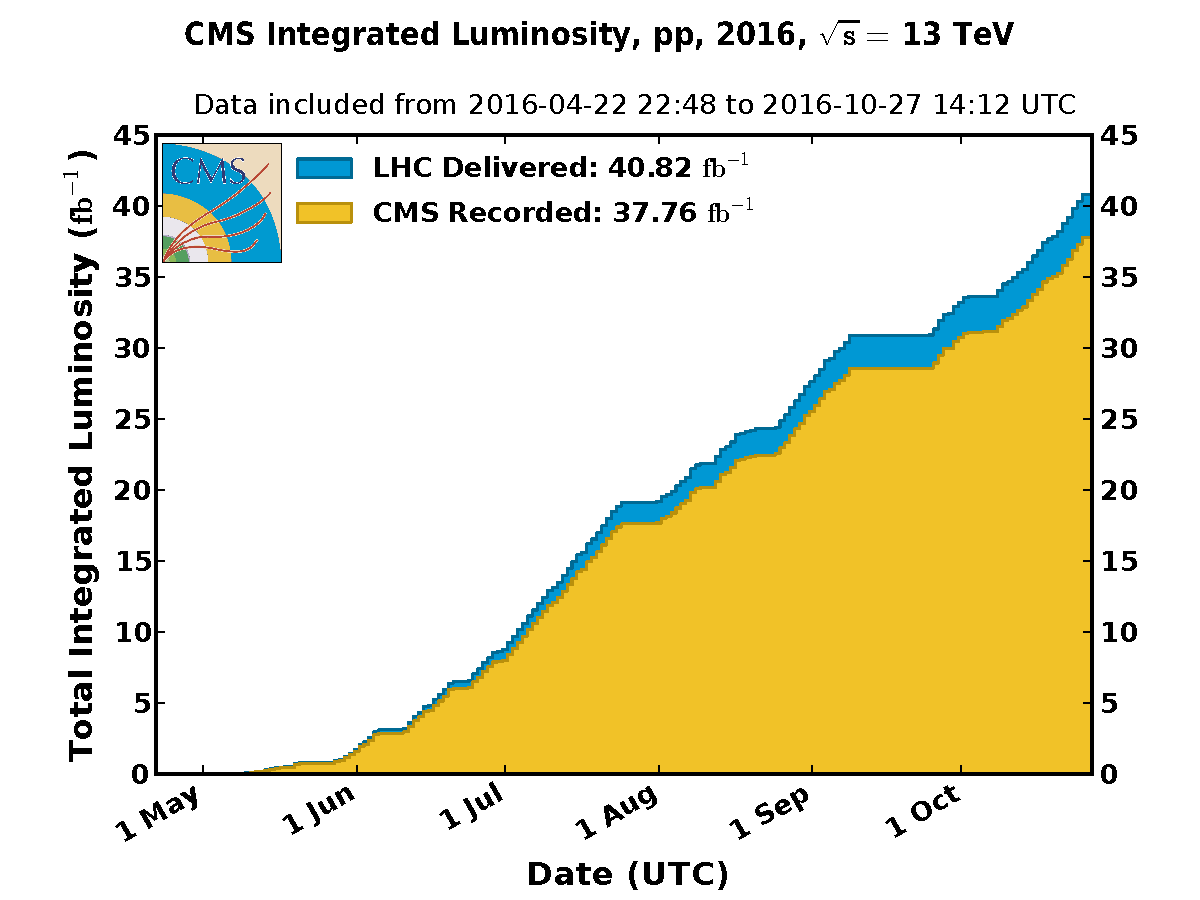
\includegraphics[width=0.7\textwidth]{pictures/int_lumi_per_day_cumulative_pp_2016.pdf}

	\caption[Total integrated luminosity of the year 2016]{Total integrated luminosity collected by \gls{CMS} in the run in the year 2016, taken from \cite{CMSLUMI}}
	\label{fig:fig_2_2}
\end{figure}


\subsection{Proton-proton collisions}
\label{sec:section_2_1_2}

Protons are non-elementary hadrons, which are a bound state of three quarks, in this case of two up-quarks and one down-quark. This bound state can be described by \gls{QCD}, see section \ref{sec:section_1_1_2}, and give rise to the quark-parton model \cite{Peskin}. In this description protons composite of the so-called partons, which are beside the three quarks of the bound state, other quarks and gluons which are produced/annihilated during the interaction in the bound state. Each of the quarks and gluons carry a fraction $x$ of the total momentum $P$ of the proton, and the probability of a existing parton with flavour f, with $f \in (u, d, \bar{u}, \bar{d}, ... g)$ and with $x$ is described by the parton density function (\gls{PDF}) $f_{f}(x)$ \cite{Peskin, PDF1}. \gls{PDF} are not predictable by \gls{QCD} and have to be measured in deep inelastic scattering processes, figure \ref{fig:fig_2_3} shows the measurement of the \gls{PDF} in the ZEUS experiment \cite{ZEUS}. \\

\begin{figure}[ht]
	\centering
	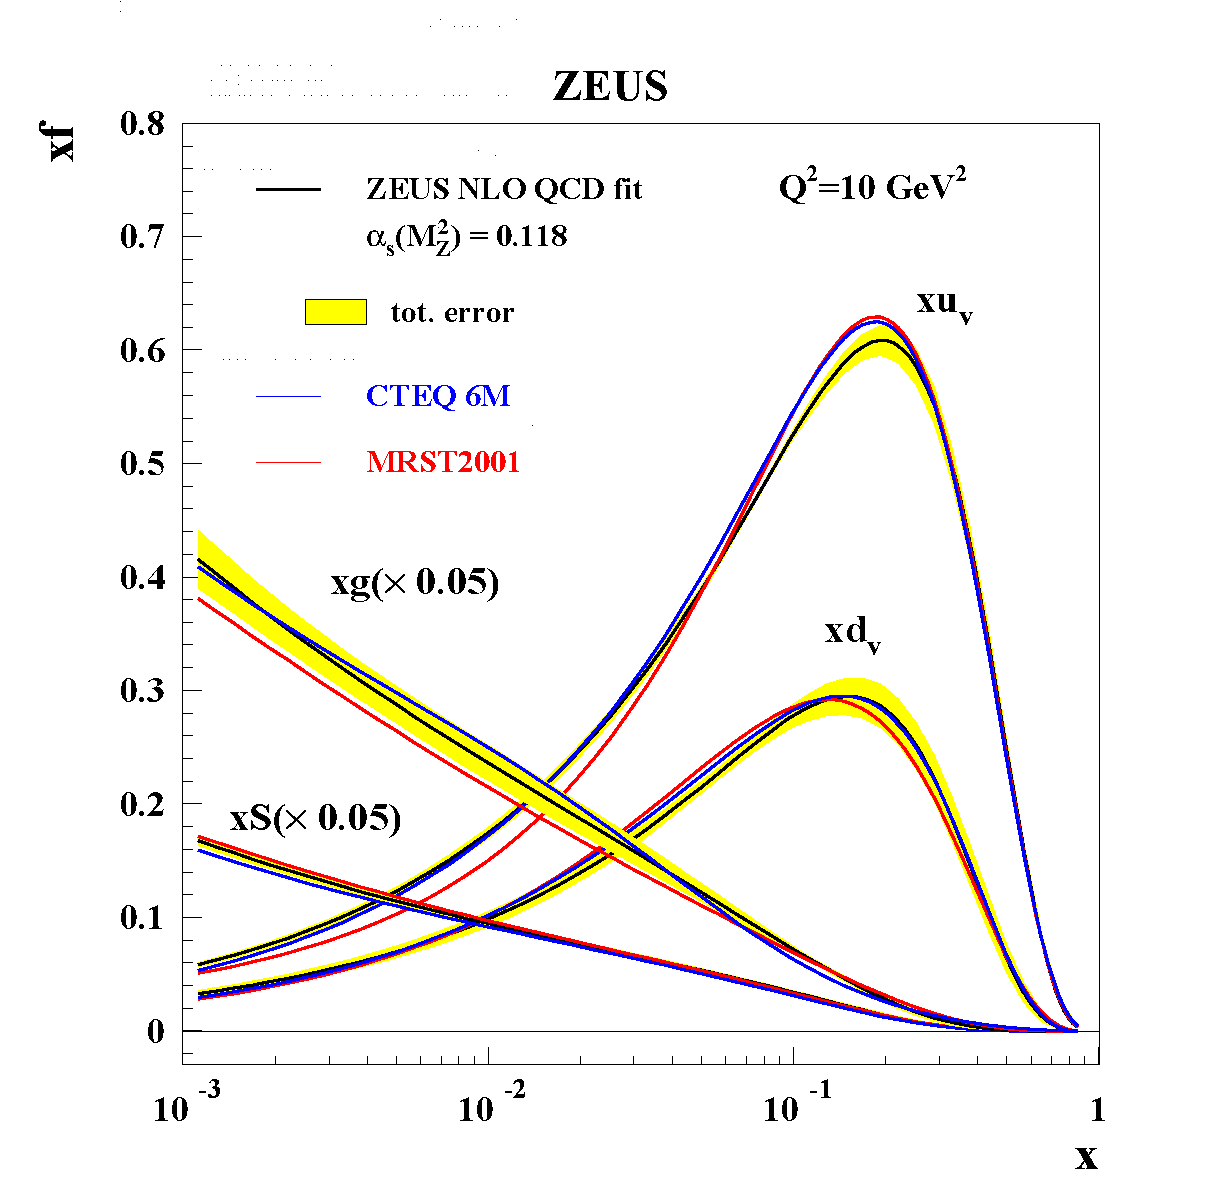
\includegraphics[width=0.7\textwidth]{pictures/ZEUS_PDF.pdf}

	\caption[Proton \gls{PDF} from ZEUS]{\gls{PDF} of up-quarks, down-quarks and gluons in a proton measured by the ZEUS experiment, taken from \cite{PDFMEAS}}
	\label{fig:fig_2_3}
\end{figure}

In collisions of the protons at the \gls{LHC} the interaction depens on the \gls{PDF} and the $x_{i}$ of the partons. Taking as example proton-proton collisions into fermion pair production, two quarks with momentum $x_{1}P$ and $x_{2}P$ will produce the fermion pair, all the other constituent $X$ are not partizipating in the interaction and carry away the remaining proton momenta, see figure \ref{fig:fig_2_4} for a schematic example. The cross section $\sigma(pp\to f\bar{f} + X)$ \cite{Peskin} for such a process in the dependence on the $x_{i}$ and the \gls{PDF} is 

\begin{equation}
	\label{eq:eq_2_3}
	\int_{0}^{1}dx_{1}\int_{0}^{1}dx_{2}\sum_{f \in (u, d, \bar{u}, \bar{d}, ... g)} f_{f}(x_{1})f_{\bar{f}}(x_{2}) \cdot \sigma(q_{f}(x_{1})q_{\bar{f}}(x_{2}) \to f\bar{f}) 
\end{equation}


\begin{figure}[ht]
	\centering
	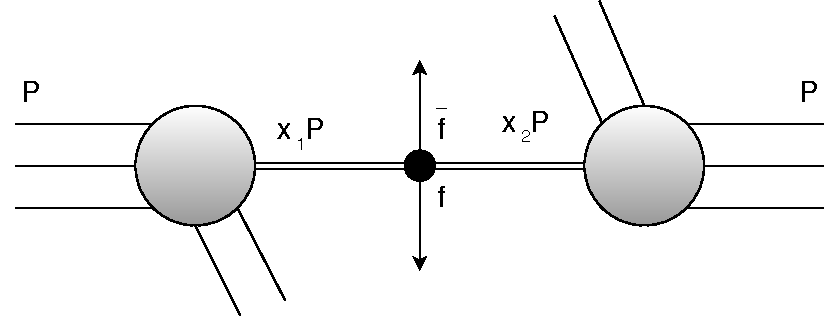
\includegraphics[width=0.7\textwidth]{pictures/ppcollision.pdf}

	\caption[Schematic sketch of proton-proton collision]{Schematic sketch of a proton-proton collision at the \gls{LHC}. The protons have momentum $P$, the quarks involved in the interaction have the fraction $x_{i}$ of it, all other rest carries away the remaining momenta}
	\label{fig:fig_2_4}
\end{figure}


\section{Compact Muon Solenoid}
\label{sec:section_2_2}

The \gls{CMS} is a multi-purpose, multi-functional particle detector. The detector consists of several layers, which have each an own functionality and purpose for the detection of particles. This design enables the measurement of kinematic proporties of the particles, like momenta/energy/angular distributions, and the identification of the particles. Figure \ref{fig:fig_2_5} shows the \gls{CMS} profile with all detector layers, which are explained in section \ref{sec:section_2_2_2}, and the particles interaction in the detector, which are explained in section \ref{sec:section_2_2_3}.

\begin{figure}[ht]
	\centering
	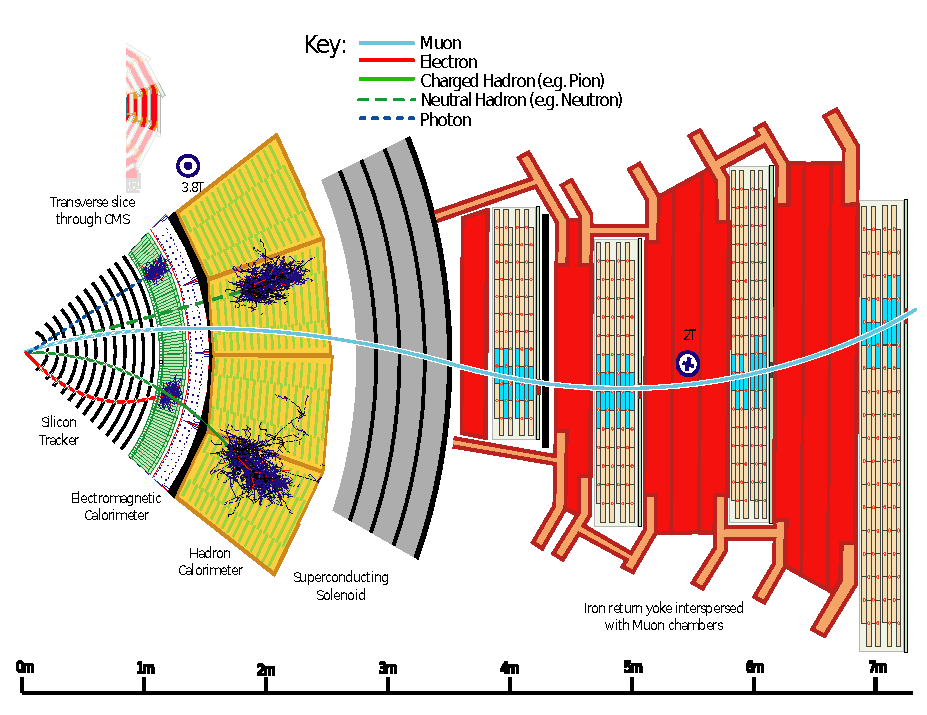
\includegraphics[width=0.7\textwidth]{pictures/CMS.pdf}

	\caption[Profile of CMS detector]{Schematic sketch of the profile of \gls{CMS} with detectors and possible particle and their interactions in the detectors, taken from \cite{PARTICLEFLOW}}
	\label{fig:fig_2_5}
\end{figure}


\subsection{Coordinate convention}

The coordinate system to describe the \gls{CMS} detector architeture is set to have the origin centered at the nominal collision point of the detector, with the x-axis pointing into the direction of the center of \gls{LHC}, the y-axis is pointing upwards into direction of the sky and z-axis points into the direction of the beam pipe. The orbital coordinate system is choosen in a way, that the azimuthal angle $\phi$ is measured in the x-y plane, and the polar angle $\theta$ is measured from the z-axis. Instead the polar angle $\theta$, in general the pseudo rapidity \gls{eta} $= -\ln{\tan{\frac{\theta}{2}}}$ is used due to the invariance of lorentz boost of $\Delta$\gls{eta} of two objects in the high energy limit.


\subsection{Components of the \gls{CMS} detector}
\label{sec:section_2_2_2}

The most inner part of \gls{CMS} is the silicon tracker system \cite{CMS2, CMSTRACKER}. The inner part of the tracker system is the pixel detector, which is cylindric build around the beam. It consists of three layers in the barrel, which are locacted at the radial distance of 4.4 cm, 7.3 cm, 10.2 cm and have a length of 53 cm, and two turbine shaped layers on each side of the barrel, which are located $|z| = 34.5/46.5$cm and have a radial expansion of 6 to 15 cm. Figure \ref{fig:fig_2_6} shows the layout of the pixel detector. All in all $66\cdot 10^{6}$ pixels with a size of 100 x 150 $\mu$m$^{2}$ are implemented in the pixel detector, which has a precision of 10 $\mu$m in the $r-\phi$ direction and a precision of 20 $\mu$m in the z direction. \\

\begin{figure}[ht]
	\centering
	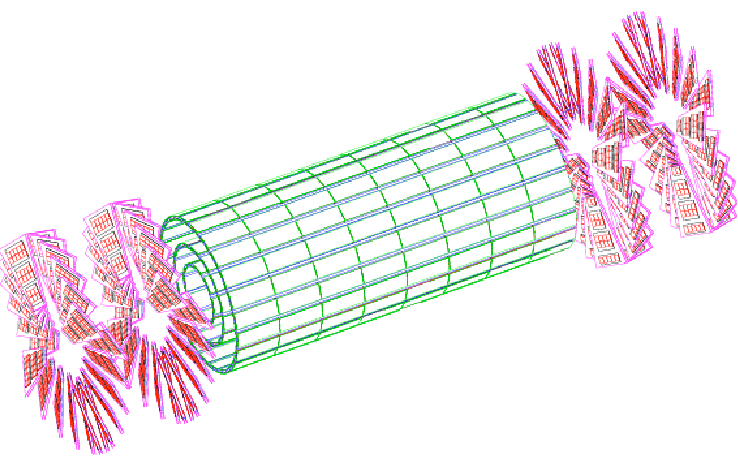
\includegraphics[width=0.7\textwidth]{pictures/CMS_tracker.pdf}

	\caption[Pixel detector layout of CMS]{Pixel detector layout of CMS, taken from \cite{CMS2}}
	\label{fig:fig_2_6}
\end{figure}


The outer part of the tracker system is the silicon strip detector. The strip detectors are spaced in cylindric layers around the beam pipe and are divided into a inner/outer barrel and the inner disc and endcap. The inner barrel is made of 4 layers with a coverage in z direction up to 65 cm in each direction, with a strip thickness of 320 $\mu$m and a $r-\phi$ resolution of 23-34 $\mu$m and z resolution of 23 $\mu$m. The outer barrel includes six layers with a strip thickness of 500 $\mu$m, a coverage in z direction up to 110 cm and a $r-\phi$ resolution of 35-52 $\mu$m and z resolution of 52 $\mu$m. The endcap are nine disc-like layers on each side in z direction, occupaying the space in the range 120cm $< |z| < $ 280cm, the inner discs are arranged in 3 layers and fill the gap between barrel and endcap. In total a \gls{eta} region up to $|$\gls{eta}$|$ $< 2.5$ is covered by the complete strip detector. Figure \ref{fig:fig_2_7} shows the layout of the strip detector. \\

\begin{figure}[ht]
	\centering
	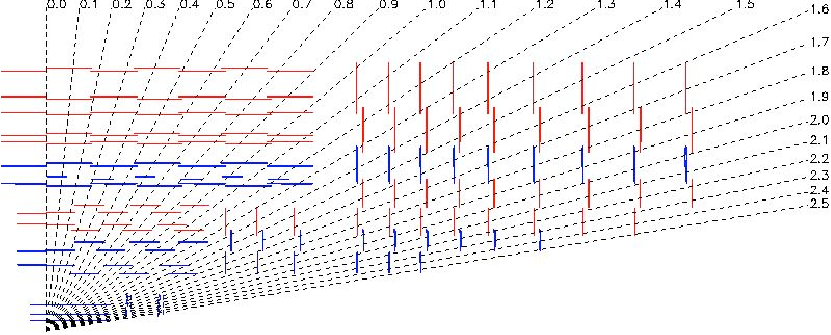
\includegraphics[width=1\textwidth]{pictures/CMS_strip.pdf}
	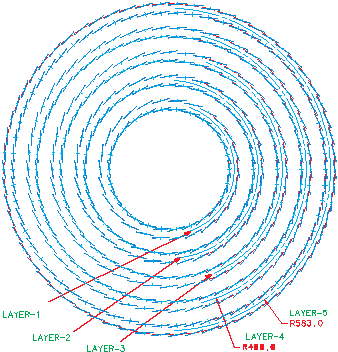
\includegraphics[width=0.5\textwidth]{pictures/CMS_strip2.pdf}

	\caption[Strip detector of CMS]{The first subfigure shows the layout in a z-view, where the numbers give the $\eta$ region. The second subfigure shows a transverse view of the barrel strip detector, takem from \cite{CMS2, ECAL}}
	\label{fig:fig_2_7}
\end{figure}

After the tracker system the calorimeter system is installed. The electromagnetic calorimeter (\gls{ECAL}) \cite{CMS2, ECAL} is build up by 61200 lead tungstate (\gls{PbWO4}) crystals in the barrel part and 7324 crystals in the endcap. The barrel region covers a region from 0 $<$ $|$\gls{eta}$|$ $<$ 1.479, in which each crystal have the dimensions of 22mm x 22mm x 230mm. The endcap region covers to remaining part of 1.479 $<$ $|$\gls{eta}$|$ $<$ 3.0, in which the crystals have a dimension of 28.6mm x 28.6mm x 220mm. In $r$ direction the barrel region is located at a distance to the beam pipe of 129 cm, the endcap region is located at a distance of 314cm. Figure \ref{fig:fig_2_8} shows the schematic view of the \gls{ECAL}. For the readout of energy deposition of the particles in the barrel region silicon avalanche photodiodes are used, in the endcap vacuum phototrides are used. The energy resolution of the \gls{ECAL} is given by

\begin{equation}
	\label{eq:eq_2_4}
	\frac{\sigma}{E} = (\frac{3.63 \sqrt{\text{MeV}}}{\sqrt{E}})^2 + (\frac{124 \text{MeV}}{\sqrt{E}})^2 + 0.26^{2}
\end{equation}

and measured for supermodules, which group 4 modules, which contains 500 crystalls each. \\

\begin{figure}[ht]
	\centering
	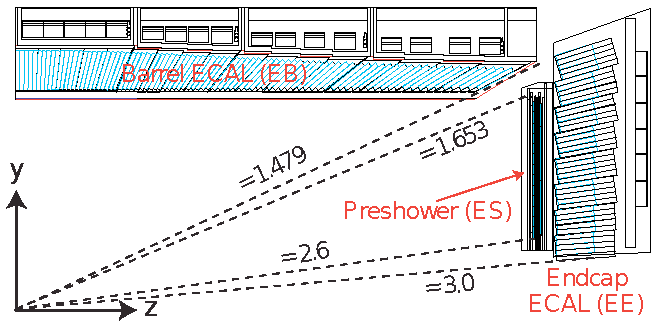
\includegraphics[width=1\textwidth]{pictures/CMS_ElectromagneticCalorimeter.pdf}

	\caption[Electromagnetic calorimeter of CMS]{Schematic view of the \gls{ECAL}, taken from \cite{CMS2}}
	\label{fig:fig_2_8}
\end{figure}

The second part of the calorimeter system is the hadronic calorimeter (\gls{HCAL}) \cite{CMS2, HCAL}. It is build up by wedges made of brass absorber plates, orientated parallel to the beam axis, with plastic scintillators between each absorber plate. The placement of absorber/scintillator is alternating, in sum 17 layers of active scintillator material is placed, which are connected with a wavelength shifting fiber, forming so-called towers. The readout of the optical signal from the HCAL towers is done by pixelated hybrid photodiodes. The \gls{HCAL} is divided into a barrel region with $|$\gls{eta}$|$ $< 1.3$, with 32 towers, and the endcap region covering the region of 1.3 $<$ $|$\gls{eta}$|$ $<$ 3.0 with 14 towers. In addition to that outer hadron calorimeter system located at the muon chambers is installed. It is assembled in 5 rings placed by a distance of 2.54 m in z-direction, covering a region of $|$\gls{eta}$|$ $< 1.24$, where the ring are made of a layer of iron and scintillator material. Figure \ref{fig:fig_2_8} shows a schematic overview of the tower assembly. \\

\begin{figure}[ht]
	\centering
	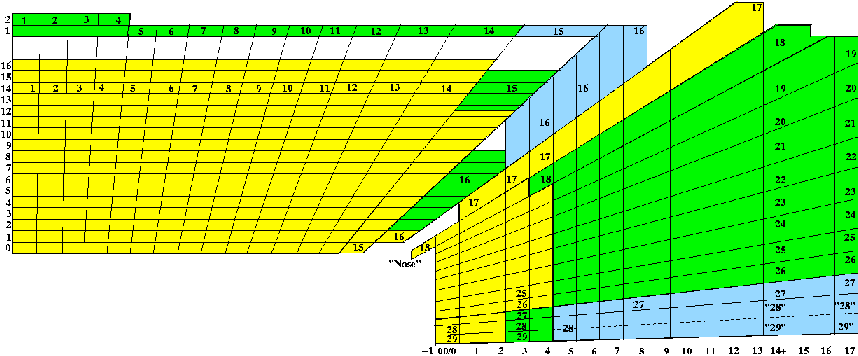
\includegraphics[width=1\textwidth]{pictures/HCAL.pdf}

	\caption[Hadronic calorimeter of CMS]{Schematic view of the towers assembly in barrel and endcap in the r-z plane of the \gls{HCAL}, taken from \cite{CMS2}}
	\label{fig:fig_2_9}
\end{figure}

The magnet field of \gls{CMS} is generated by superconducting coils made of aluminium, which has a inner diameter of 6.22 m and a length of 13.48. The coil is enclosed in iron yokes, which gives rise to a magnetic field of 4 Tesla. The barrel part of the iron yoke is 11 long and divided into five rings with a distance of 2.5 along the beam axis, and has a material weight of 6000 tonnes. The end cap of the iron jokes is made of three disk at each side of the detector with a weight of 4600 tonnes.

The most outer detector component is the muon detector system, which is embedded in the iron yoke. The muon system itself relies for the muon detection on three types of gaseous detectors, the drift tubes, the cathode strip chambers and the resistive plate chambers. In the barrel region, covering the region $|$\gls{eta}$|$ $< 1.2$, 250 drift tube chambers organized in four layers with a distance to the beam pipe of 4-7 meters are installed. To the drift tubes 1 or 2 resistive plates chamber are coupled depending on the layer. The endcap region of the system, convering the region of $|$\gls{eta}$|$ $< 2.4$, 468 cathode strip chambers are installed in both sides of the detector, which are assembled in 4 rings. In the region of $|$\gls{eta}$|$ $< 1.6$  resistive plates chamber are coupled to the cathode strip chambers. Figure \ref{fig:fig_2_10} shows a overview of the muon system.

\begin{figure}[ht]
	\centering
	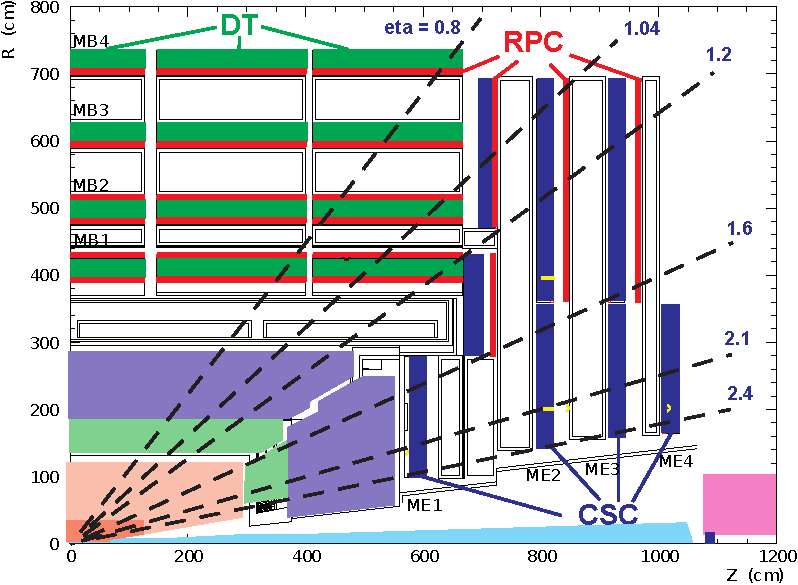
\includegraphics[width=1\textwidth]{pictures/MUON_SYSTEM.pdf}

	\caption[Muon detector system of CMS]{Schematic view of the muon detector system of the r-z plane, where the drift tubes are drawn in green, the resistive plates chamber are drawn in red and the cathode strip chambers are drawn in blue. Taken from \cite{CMS2}}
	\label{fig:fig_2_10}
\end{figure}


\subsection{Trigger system of \gls{CMS}}

The collision rate at the collision point of \gls{CMS} is about 40 Gigahertz, coming from the 25 ns space between the beam bunches, see section \ref{sec:section_2_1_1}. This collision rate leads at the luminosity of $\mathcal{L} = 10^{34}$ cm$^{-2}$s$^{-1}$ to a interaction rate of $10^9$ per second. Because the bare amount of data originating from this collisions can not completly be saved, a online selection is done by the \gls{CMS} trigger system \cite{CMS2, TRIGGER}. \\

The first trigger stage is the L1 trigger. This decision of this trigger is taken from the information various local trigger from the detector subsystem, which uses all information recorded of the event. The second stage is the High Level Trigger \gls{HLT}. Based on the events passing the L1 trigger, the \gls{HLT} decide to keep events on behalf of kinematic variables, which are reconstructed online during the trigger decision. 

\subsection{Particle interactions with the detector components}
\label{sec:section_2_2_3}

The dectector components described in the previous section are designed to detect and measure different properties of the particles. Charged particle, like leptons and charged hadrons, have bended trajectory in the in magnetic field of \gls{CMS} and leaving hits in the pixel and strip detectors of the tracker system. Neutral particles like photons and neutral hadrons dont leave any track in the tracker system and have a straight trajectory. In the \gls{ECAL} electrons and photons interact with the \gls{PbWO4} and trigger a electromagnetic shower, until the complete energy is deposited. In the \gls{HCAL} all kind of hadrons interact with the bress triggering a cascade of hadron production, until the complete energy is deposited. The muons, which penetrate all this system without any interaction, leave hits in the muon detector system. Neutrinos can not be measured at all and escape the complete dectector system undetected. \\

The cascade of particles in the calorimeter systems, which originating from one object, like a quark or gluon, are so-called jets. There are different algorithm to define and reconstruct jets in \gls{CMS} using the definition of a cone with \gls{dR} $= \sqrt{(\Delta \phi)^{2} + (\Delta \eta)^{2}}$.\\ 

From the bending radius of the particles and in tracker system and for the muons in the muon detector system, the transerve momentum \gls{pT} $= \sqrt{p_{x}^{2} + p_{y}^{2}}$ can be measured using 

\begin{equation}
	\label{eq:eq_2_5}
	p_{T} = q\cdot B \cdot R
\end{equation} 

with $q$ as the electric charge of the particle, $B$ the magnetic field flux and R the bending radius of the trajectory. The energy of particles is measured using the energy deposition in the calorimeter systems. Due to neutrinos and possible \gls{BSM} weakly interacting particles, some energy gets carries away unmeasured. This missing energy measured in the transverse plane (\gls{MET}) is calculated using the fact that in the transverse plane the sum of the momenta should be zero, due to the protons only having momenta in z-direction. This leads to the formula for \gls{MET}

\begin{equation}
	\label{eq:eq_2_6}
	\vec{E}_{T}^{\text{miss}} = - \sum_{i \in (1, .., n_{\text{meas.}})} \vec{p}_{T}^{i} 
\end{equation}

Unstable particles, which decay not immediately, like the $\tau$ lepton, leave a track in the tracker system with a sudden change of direction. At this so-called secondary vertex the $\tau$ lepton decays, for example into a muon and two neutrinos, where the muon leaves the track measured originating from the second track. To characterize the properties of the particles coming from secondary vertices, the trajectory is extrapolated beyond the secondary vertex and the point of closest approach $d_{0}$ is measured of this extrapolated trajectory and the colission point, see figure \ref{fig:fig_2_11}.

\begin{figure}[ht]
	\centering
	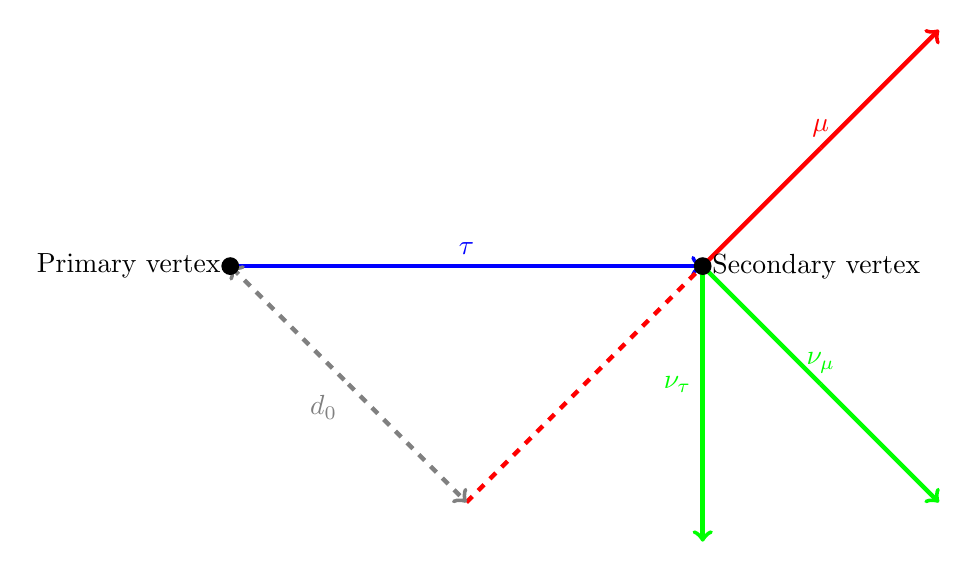
\begin{tikzpicture}
		\draw[blue, ultra thick] (-6,0) -- (-3,0) node[anchor=south] {$\tau$};
		\draw[->, blue, ultra thick] (-6,0) -- (0,0);
		\draw[red, ultra thick] (0,0) -- (1.5,1.5) node[anchor=south] {$\mu$};
		\draw[->, red, ultra thick] (1.5,1.5) -- (3,3);
		\draw[green, ultra thick] (0,0) -- (1.5,-1.5) node[anchor=south] {$\nu_{\mu}$};
		\draw[->, green, ultra thick] (1.5,-1.5) -- (3,-3);
		\draw[green, ultra thick] (0,0) -- (0,-1.5) node[anchor=east] {$\nu_{\tau}$};
		\draw[->, green, ultra thick] (0,-1.5) -- (0,-3.5);
		\draw[red, ultra thick, dashed] (-3,-3) -- (0,0);
		\draw[<-, gray, ultra thick, dashed] (-6,0) -- (-4.5,-1.5) node[anchor=north east] {$d_0$};
		\draw[->, gray, ultra thick, dashed] (-4.5,-1.5) -- (-3,-3);
		\filldraw[black] (-6,0) circle (3pt) node[anchor=east] {Primary vertex};
		\filldraw[black] (0,0) circle (3pt) node[anchor=west] {Secondary vertex};
	\end{tikzpicture}
	\caption[Construction of point of closest approach]{Construction for measuring the point of closest approach $d_{0}$ of the muon trajectory to the collision point}
	\label{fig:fig_2_11}
\end{figure}


